\begin{figure}[!t]
\centering
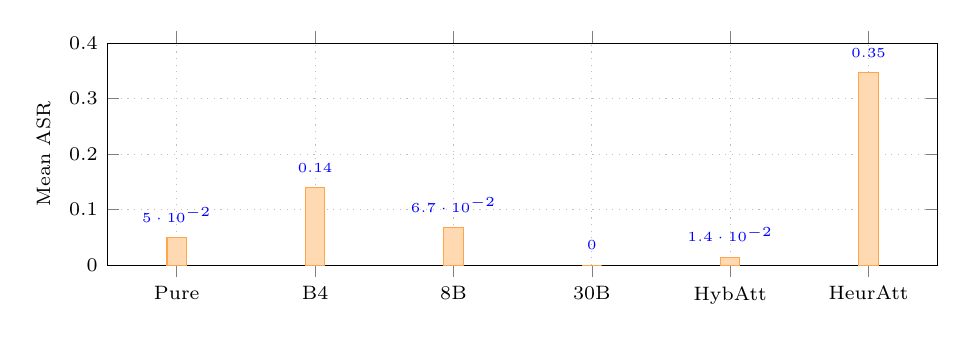
\begin{tikzpicture}
\begin{axis}[
  ybar,
  bar width=7pt,
  width=\columnwidth,
  height=4.4cm,
  ymin=0, ymax=0.40,
  ylabel={Mean ASR},
  symbolic x coords={Pure, B4, 8B, 30B, HybAtt, HeurAtt},
  xtick=data,
  xticklabel style={font=\scriptsize},
  yticklabel style={font=\scriptsize},
  label style={font=\scriptsize},
  grid=major,
  major grid style={dotted,gray!50},
  nodes near coords={\pgfmathprintnumber[precision=2]{\pgfplotspointmeta}},
  every node near coord/.append style={font=\tiny, yshift=2pt},
]
\addplot+[fill=orange!30, draw=orange!70] coordinates {
(Pure, 0.050)
(B4, 0.139)
(8B, 0.067)
(30B, 0.000)
(HybAtt, 0.014)
(HeurAtt, 0.347)
};
\end{axis}
\end{tikzpicture}
\caption{Supplementary language-model conditions (two or three seeds
each). Pure LLM and hybrid attacker against a heuristic defender stay near
zero; a heuristic attacker against a hybrid defender reaches the highest
mean ASR; model scale is non-monotonic (8B vs.\ 30B).}
\label{fig:llm-ablation}
\end{figure}
